\documentclass[a0,portrait,final]{a0poster}
% You might find the 'draft' option to a0 poster useful if you have
% lots of graphics, because they can take some time to process and
% display. (\documentclass[a0,draft]{a0poster})

% Switch off page numbers on a poster, obviously, and section numbers too.
\pagestyle{empty}
\setcounter{secnumdepth}{0}

% The textpos package is necessary to position textblocks at arbitary 
% places on the page.
\usepackage[absolute]{textpos}

% Graphics to include graphics. Times is nice on posters, but you
% might want to switch it off and go for CMR fonts.
\usepackage{graphics,wrapfig,times}

% These colours are tried and tested for titles and headers. Don't
% over use color!
\usepackage{color}
\definecolor{darkblue}{rgb}{0.1,0.1,0.5}
\definecolor{darkred}{rgb}{0.8,0.0,0.1}

% see documentation for a0poster class for the size options here
%\let\Textsize\normalsize
%\def\Head#1{\noindent\hbox to \hsize{\hfil{\LARGE\color{darkblue} #1}}\bigskip}
%\def\LHead#1{\noindent{\LARGE\color{darkblue} #1}\smallskip}
%\def\Subhead#1{\noindent{\large\color{darkblue} #1}}
%\def\Title#1{\noindent{\VeryHuge\color{darkred} #1}}

% Set up the grid
%
% Note that [40mm,40mm] is the margin round the edge of the page --
% it is _not_ the grid size. That is always defined as 
% PAGE_WIDTH/HGRID and PAGE_HEIGHT/VGRID. In this case we use
% 15 x 25. This gives us a wide central column for text (7 grid
% spacings) and two narrow columns (3 each) at each side for 
% pictures, separated by 1 grid spacing.
%
% Note however that texblocks can be positioned fractionally as well,
% so really any convenient grid size can be used.
%
\TPGrid[40mm,40mm]{15}{25}  % 3 - 1 - 7 - 1 - 3 Columns

% Mess with these as you like
\parindent=0pt
\parskip=1.0\baselineskip
%\renewcommand{\baselinestretch}{0.95}


%\usepackage{amsmath,amsthm, amssymb, latexsym}
\usepackage{fix-cm}
\usepackage[english]{babel}
\usepackage[latin1]{inputenc}
\usepackage{times}
\usepackage[T1]{fontenc}
\usepackage{calc} 

% PGF includes
\usepackage{pgf}
\usepackage{tikz}
\usetikzlibrary{shadows,calc,plotmarks}
\usetikzlibrary{shapes,arrows}
\pgfdeclarelayer{background}
\pgfdeclarelayer{foreground}
\pgfsetlayers{background,main,foreground}
%\usetikzlibrary{,decorations,backgrounds,matrix,automata,trees,shapes,}

%%%%%
\newcommand{\posterheading}[1]{
	\begin{center}
	  \begin{tikzpicture}
		\definecolor{darkblue}{rgb}{0.1,0.1,0.5}
		\node [draw=none,rounded corners=1ex, 
			minimum height=7ex, minimum width=0.95\columnwidth, 
			top color= darkblue!40, bottom color= darkblue!70]
			%top color= black!40, bottom color=black!70]
			{
				\color{white}{\huge #1}
			};
	  \end{tikzpicture}
	\end{center}
}

\newcommand{\postertitle}[3]{
	\begin{center}
	  \begin{tikzpicture}
		\definecolor{darkblue}{rgb}{0.1,0.1,0.5}
		\node [draw=none,rounded corners=3ex, 
			minimum height=40ex, minimum width=\columnwidth]
			{
				\begin{tabular}{c}
				\color{black}{\bf \VeryHuge #1}\\ \\
				\color{darkblue}{\Huge #2}\\ \\
				\color{darkblue}{\LARGE {#3}}\\
				\end{tabular}
			};
	  \end{tikzpicture}
	\end{center}
}

\newcommand{\alert}[1]{{\color{darkred}{#1}}}
\renewcommand{\normalsize}{\Large}
%%%%%

\begin{document}

%%%%% Header
\begin{textblock}{15}(0,-0.5)
\postertitle
{Learning Context Conditions for BDI Plan Selection}
{Dhirendra~Singh$^1$~~~
Sebastian~Sardina$^1$~~~
Lin~Padgham$^1$~~~
St\'ephane~Airiau$^2$}
{\begin{tabular}{c}
	$^1$School of Computer Science \& Information Technology, 
	RMIT University, Australia\\
	$^2$Institute for Logic, Language and Computation, 
	University of Amsterdam, The Netherlands
\end{tabular}}
\end{textblock}


%%%%% Introduction
\begin{textblock}{4.6}(0.2,4)
\posterheading{Summary}
We address the \alert{plan selection problem} in Belief, Desire, Intentions (BDI) Ag\-ent Systems.

%An important drawback in BDI is the lack of a learning ability. 
\alert{Context conditions} of plans determine
applicability in given situations, and must be specified
\begin{wrapfigure}{l}{0.48 \columnwidth}
  \vspace{-0.2em}
  \begin{center}
    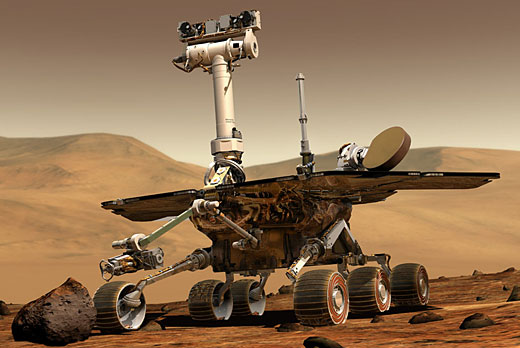
\includegraphics[width=0.45\columnwidth]{figs/mars_rover.jpg}
  \end{center}
  \vspace{-0.5em}
\end{wrapfigure}
upfront. However, new environments often require learning changes to selection conditions.


Easing this constraint would allow conditions to be \alert{refined} once deployed, improving adaptability. 

Our learning framework augments plan's context conditions with \alert{decision trees}, allowing \alert{plan applicability} to be learnt from experience.

Using a \alert{probabilistic plan selection} function, the agent balances exploration and exploitation of plans, while learning online.
\end{textblock}

%%%%% BDI Plan Library
\begin{textblock}{4.6}(0.2,13)
\posterheading{BDI Architecture}

A \alert{plan} is a rule of the form $e: \psi \leftarrow \delta$; program $\delta$ is a strategy for goal $e$ when context $\psi$ holds.

The burden for the programmer is to perfectly design the logical formula $\psi$.

\vskip 1.0em
\begin{center}
%!TEX root = ../dsingh-aamas10-poster.tex
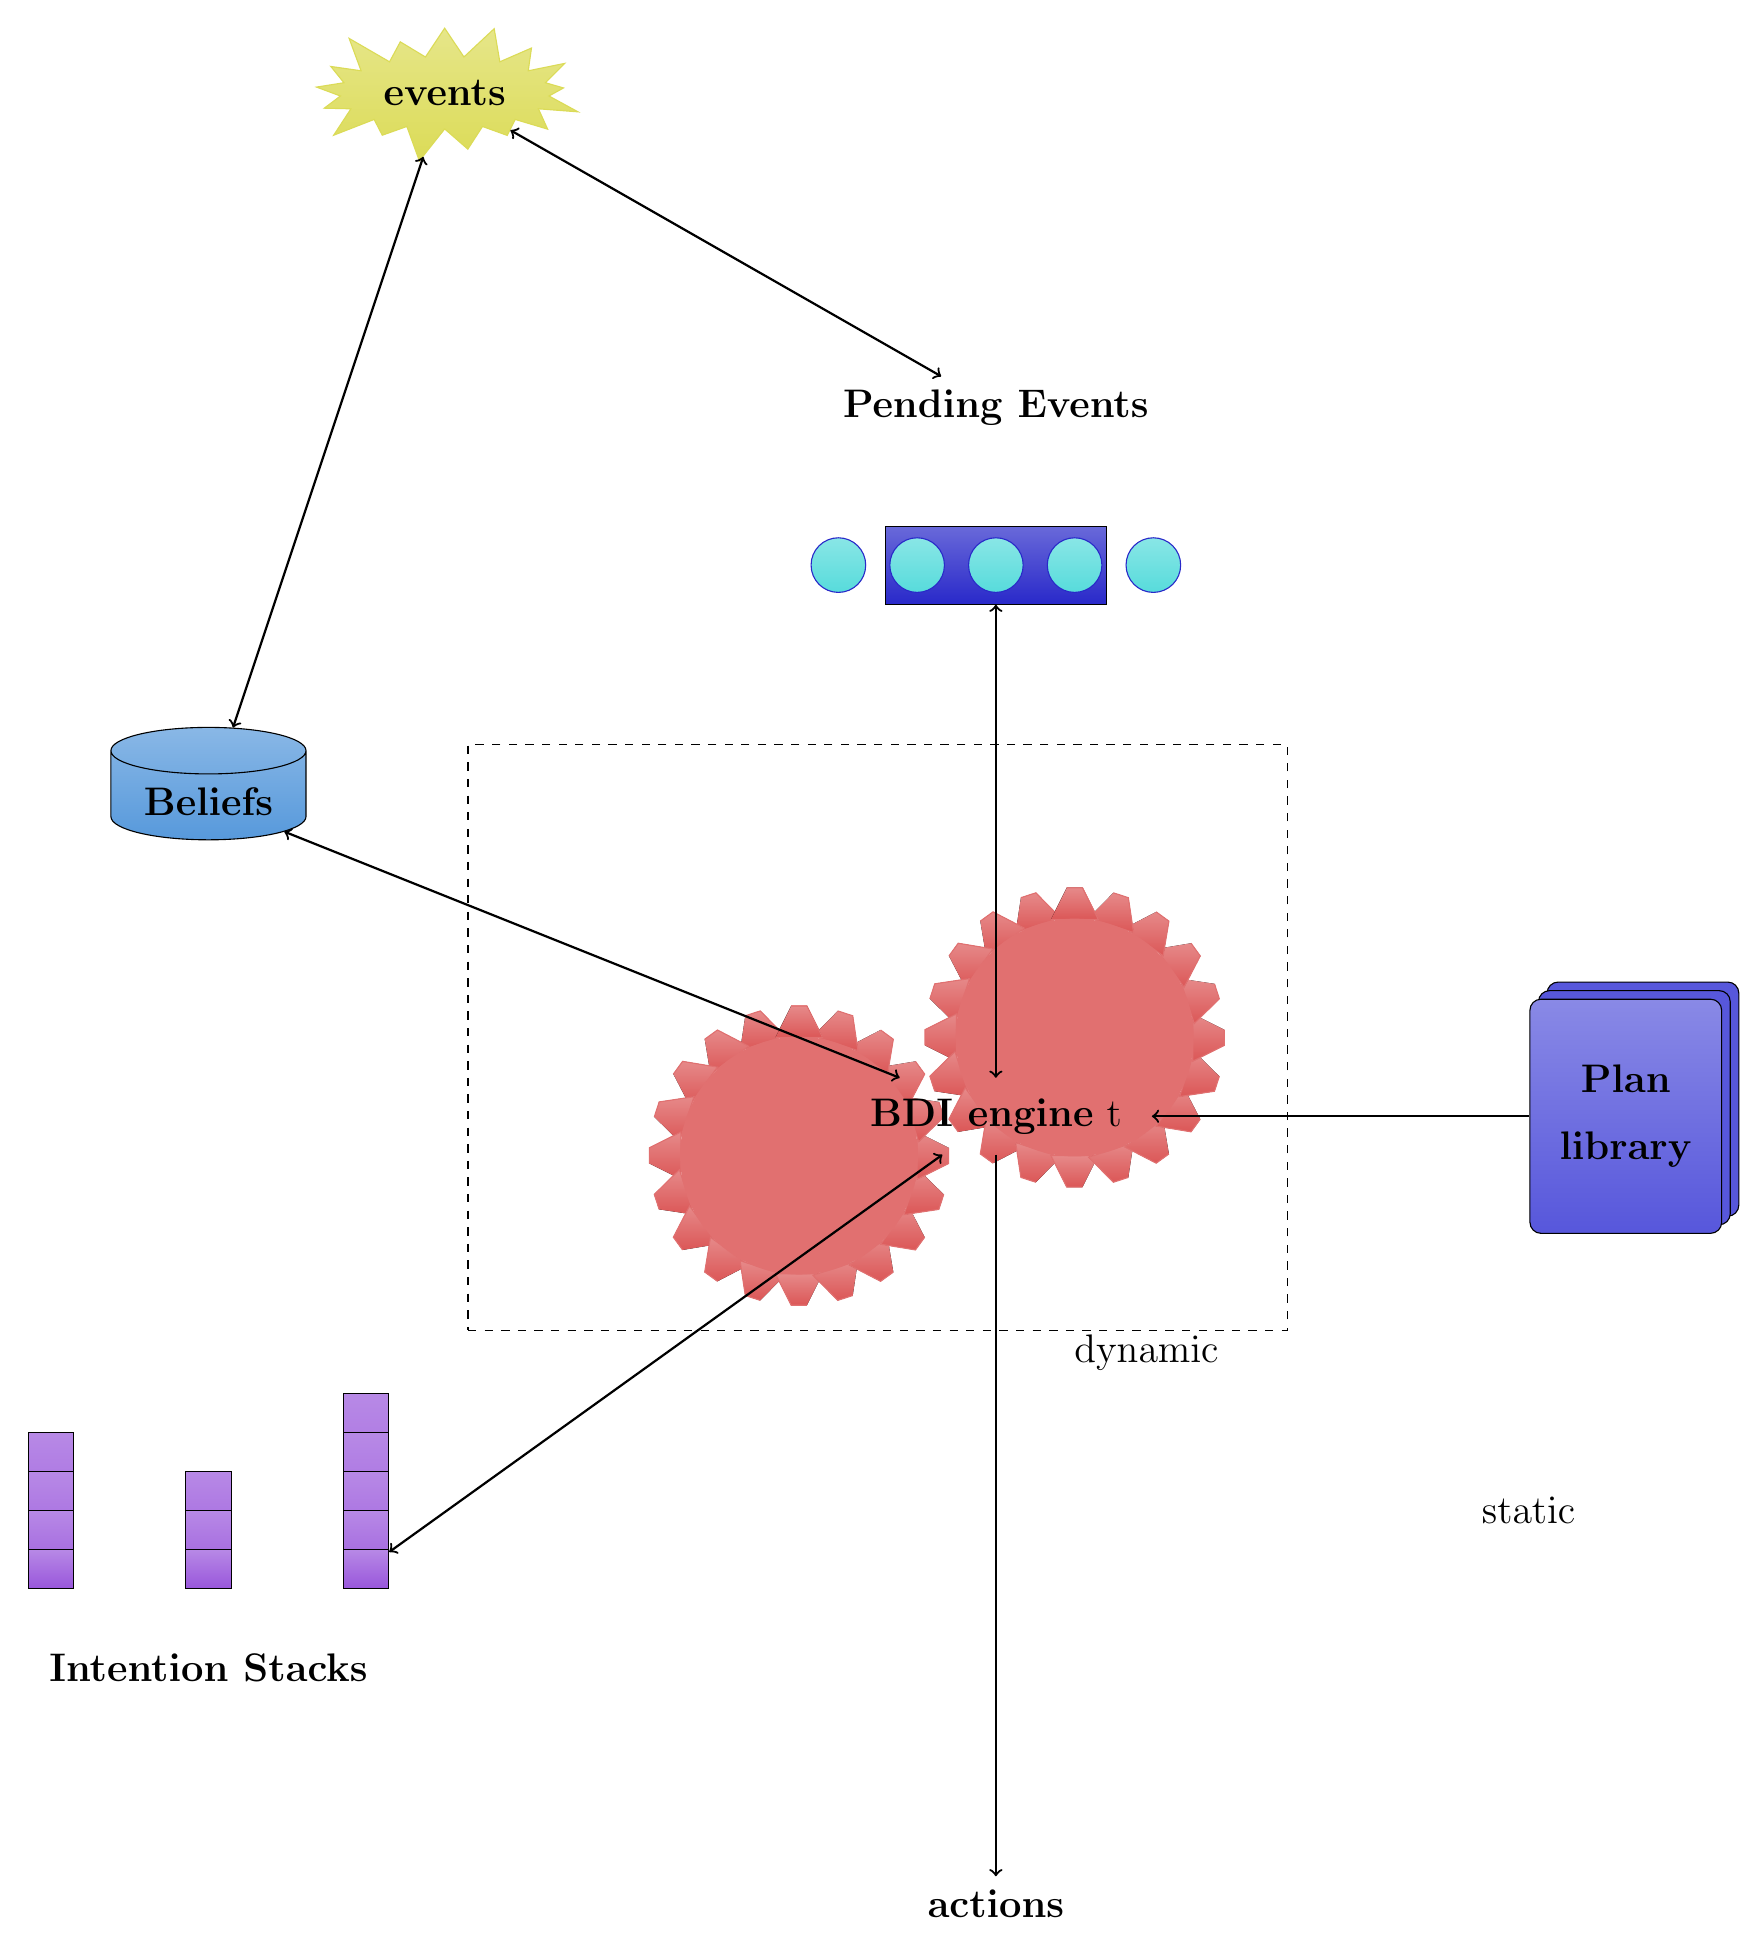
\begin{tikzpicture}

\definecolor{green1}{rgb}{0.86,0.86,0.34}
\definecolor{red1}{rgb}{0.86,0.34,0.34}
\definecolor{blue5}{rgb}{0.6,0.34,0.86}
\definecolor{blue4}{rgb}{0.16,0.16,0.79}
\definecolor{blue3}{rgb}{0.34,0.86,0.86}
\definecolor{blue2}{rgb}{0.34,0.6,0.86}
\definecolor{blue1}{rgb}{0.34,0.34,0.86}

\tikzstyle{centityd}=[draw=black]
\tikzstyle{centityf}=[fill=blue1!30]
\tikzstyle{centity}=[centityd,centityf]
\tikzstyle{entity}=[centity,thick,text centered,anchor=center]



%%% Beliefs
\node (database) at (-3,10)  (B)
	[draw=black,top color=blue2!70, bottom color=blue2,cylinder,shape border rotate=90,minimum width=5em,shape aspect=.3]
	{\textbf{Beliefs}};


%%% Pending Events
\node at (7,15) (eventQueue) {{\bf Pending Events}};
\begin{pgfonlayer}{foreground}
\foreach \x in {5,6,...,9}
\draw [draw=blue4,top color=blue3!70, bottom color=blue3](\x,13) circle (.7em);
\end{pgfonlayer}
\draw (7,13) node (Q) 
	[draw=black,top color=blue4!70, bottom color=blue4,text width=5em, minimum height=2em] {};

%%% Plan Library
\node at (15,6)(P) 
	[draw=black,top color=blue1!70, bottom color=blue1,
	rounded corners, double copy
	shadow={fill=blue1},text centered, 
	minimum height=6em] 
	{	\begin{tabular}{c} 
          \textbf{Plan} \\[1ex]
          \textbf{library}
         \end{tabular}	};
\node[anchor=west] at (13,1) {static};

%%% Intention Stacks
\foreach \x in {4,3,2,1}
\draw (-5,0) node (I) [anchor=south,draw=black,top color=blue5!70, bottom color=blue5,text width=0.5em,
	minimum height=\x em]{};
\foreach \x in {3,2,1}
\draw (-3,0) node (I) [anchor=south,draw=black,top color=blue5!70, bottom color=blue5,text width=0.5em,
	minimum height=\x em]{};
\foreach \x in {5,4,3,2,1}
\draw (-1,0) node (I) [anchor=south,draw=black,top color=blue5!70, bottom color=blue5,text width=0.5em,
	minimum height=\x em]{};
\node at (-3,-1) (Intentions) {{\bf  Intention Stacks}};

%%% BDI Engine
\foreach \x in {0,18,...,360}
\fill [rotate around={\x:(4.5,5.5)}, draw=red1!85, top color=red1!70,bottom color=red1] 
	(4.2,7.0) -- (4.8,7.0) -- (4.6,7.4) -- (4.4,7.4);
\fill [fill=red1!85] (4.5,5.5) circle (1.51);

\foreach \x in {0,18,...,360}
\fill [rotate around={\x:(8.0,7.0)}, draw=red1!85, top color=red1!70,bottom color=red1] 
	(7.7,8.5) -- (8.3,8.5) -- (8.1,8.9) -- (7.9,8.9);
\fill [fill=red1!85] (8.0,7.0) circle (1.51);

\node[anchor=east] at (10,3)  {dynamic};

%%% Events
\node at (0,19) [starburst,draw=green1,top color=green1!70, bottom color=green1] (in) {{\bf events}};

%%% Labels and Arrows
\begin{pgfonlayer}{foreground}
\node[anchor=center] at (7,6)  (deli) 
	{\begin{tabular}{c}
     	\textbf{BDI engine} t
     \end{tabular}};
\node at (7,-4) (actions) {{\bf actions}};
\draw[thick,->] (deli) -- (actions) ; 
\draw[thick,<->] (deli) -- (I) ; 
\draw[thick,<->] (deli) -- (B) ; 
\draw[thick,<-] (deli) -- (P) ;
\draw[thick,<->] (deli) -- (Q) ; 
\draw[thick,<->] (in) -- (eventQueue) ; 
\draw[thick,<->] (in) -- (B) ; 
\end{pgfonlayer}

%%% Encapuslating box
\begin{pgfonlayer}{background}
\node[draw,dashed,rectangle,minimum height=15em,minimum width=21em ] at (5.5,7){};
\end{pgfonlayer}


\end{tikzpicture}
\end{center}
\vskip -0.3em

Plans perform primitive actions or post sub-goals that are handled in a \alert{hierarchical} manner.



\end{textblock}



%%%%% Learning Task
\begin{textblock}{4.6}(5.2,4)
\posterheading{Learning Task}
\vskip 1.0em
\begin{center}
\resizebox{\columnwidth}{!}{
%!TEX root = ../aamas11storage.tex
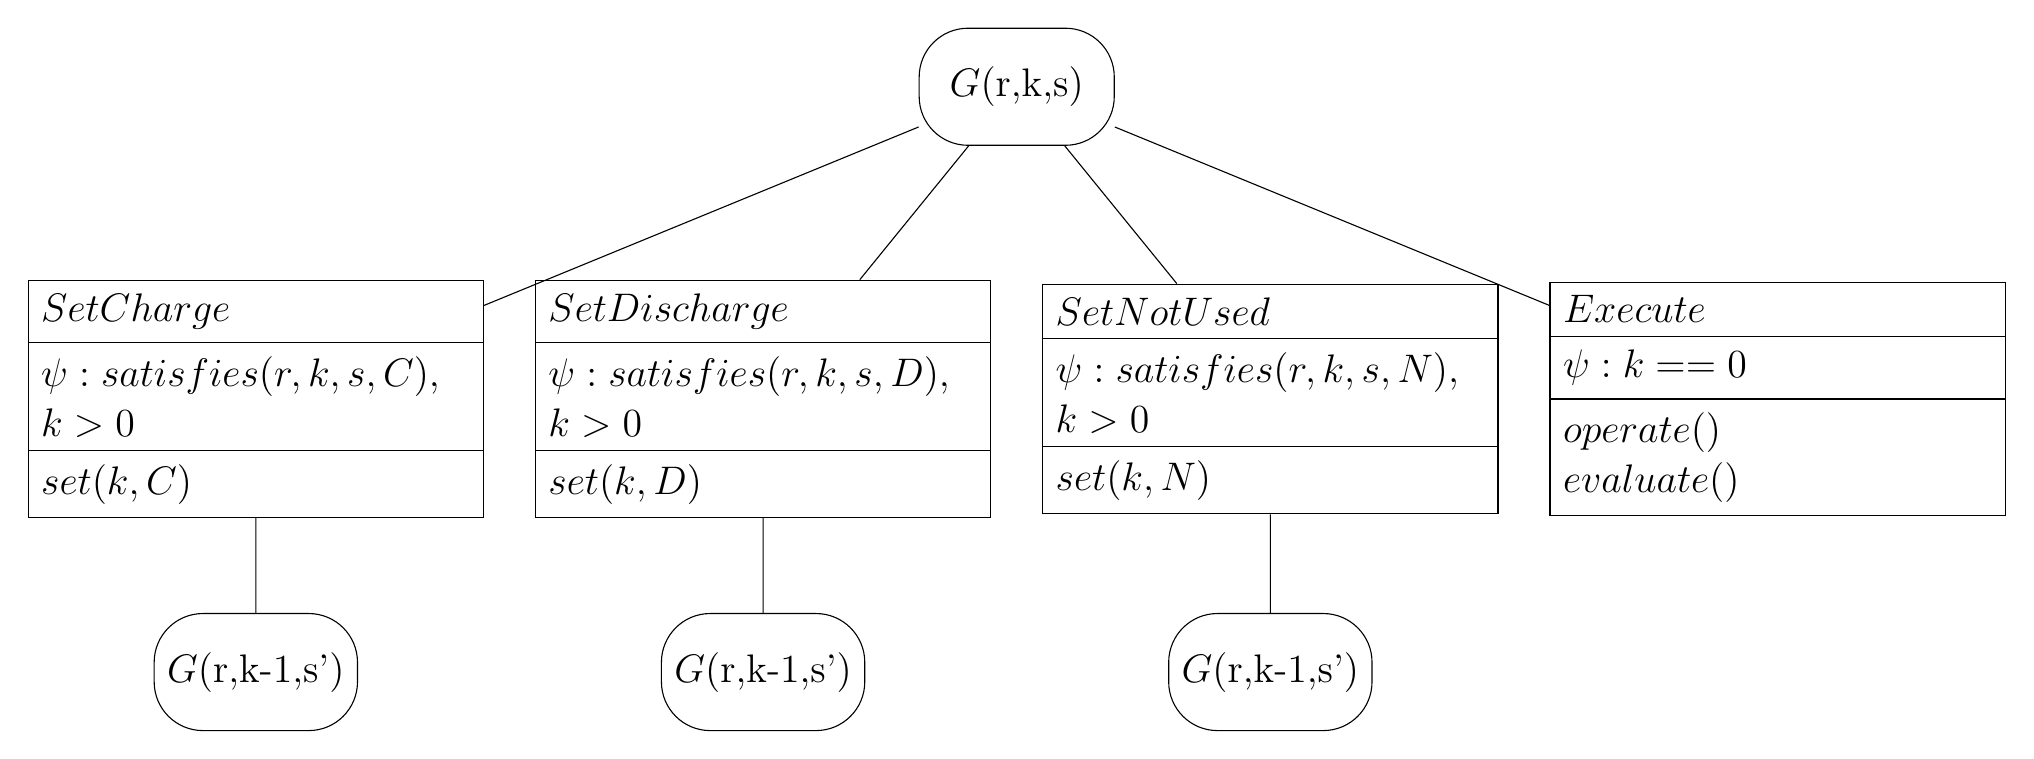
\begin{tikzpicture} [level distance=8.0em]
\tikzstyle{planbox}=[draw,text width=11.0em,rectangle split,rectangle split parts=3]
\tikzstyle{goalbox}=[draw,rounded corners=1.25em,minimum height=3em,minimum width=5em]

	
\tikzstyle{level 1}=[sibling distance=13.0em] 
\tikzstyle{level 2}=[level distance=7.0em] 

\node[goalbox,solid] {$G($r,k,s$)$}
	child {node[planbox] {$SetCharge$ 
			\nodepart{second} $\psi:satisfies(r,k,s,C),$\\$k>0$
			\nodepart{third} $set(k,C)$
		}
		child {node[goalbox] {$G($r,k-1,s'$)$}}
	}
	child {node[planbox] {$SetDischarge$ \nodepart{second}
			\nodepart{second} $\psi:satisfies(r,k,s,D),$\\$k>0$
			\nodepart{third} $set(k,D)$
		}
		child {node[goalbox] {$G($r,k-1,s'$)$}}
	}
	child {node[planbox] {$SetNotUsed$ \nodepart{second}
			\nodepart{second} $\psi:satisfies(r,k,s,N),$\\$k>0$
			\nodepart{third} $set(k,N)$
		}
		child {node[goalbox] {$G($r,k-1,s'$)$}}
	}
	child {node[planbox] {$Execute$ 
			\nodepart{second} $\psi:k==0$
			\nodepart{third} $operate()$ \\$evaluate()$
		}
	}
;

\end{tikzpicture}



}
\end{center}
\vskip 0.5em

\begin{enumerate}
\item The imposed BDI hierarchy implies that high level plans may fail not because they were poor choices for the situation but due to poor choices further below. 
\item Learning is performed \alert{online} while acting in the environment, so care must be taken in how much \alert{confidence} to put in each decision tree on an ongoing basis.

\end{enumerate}

\end{textblock}

%%%%% BDI Learning Framework
\begin{textblock}{4.6}(5.2,14)
\posterheading{BDI Learning Framework}

Each plan's logical formula context condition is augmented with a \alert{decision tree}.

A \alert{probabilistic plan selection function} balances exploitation of ongoing decision tree learning and further exploration of the state space. 

\vskip 2.0em
%\resizebox{\columnwidth}{!}{
\begin{center}
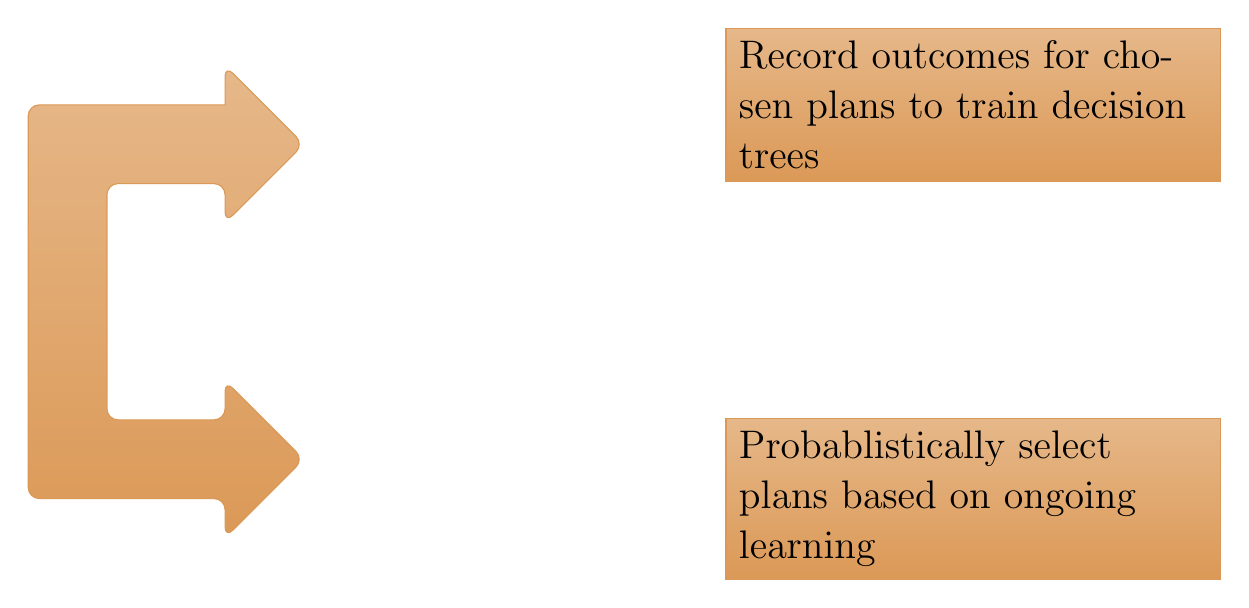
\begin{tikzpicture}
\definecolor{brown3}{rgb}{0.86,0.6,0.34}
	\node [text width=12em, draw=brown3, 
	top color=brown3!70, bottom color=brown3] at (0,0) (A) {
		Record outcomes for chosen plans to train decision trees
	};
	\node [text width=12em, draw=brown3, 
	top color=brown3!70, bottom color=brown3] at (0,-5) (B) {
		Probablistically select plans based on ongoing learning
		};
	\draw [rounded corners,brown3,top color=brown3!70, bottom color=brown3](-9.5,0) -- (-12,0) -- (-12,-5) -- (-9.5,-5) --
	(-9.5,-5.5) -- (-8.5,-4.5) -- (-9.5,-3.5) -- (-9.5,-4.0) --
	(-11,-4) -- (-11,-1) -- (-9.5,-1) -- 
	(-9.5,-1.5) -- (-8.5,-0.5) -- (-9.5,0.5) -- (-9.5,0)
	;
\end{tikzpicture}
\end{center}
%}
\vskip 0.5em
\alert{Acting and learning are interleaved}. Ongoing learning impacts the choice of future actions that impact subsequent learning and whether a good solution is eventually found.

\end{textblock}

%%% Experimentation
\begin{textblock}{4.6}(10.2,4)
\posterheading{Experimentation}

%We experiment with a range of \alert{synthetic hierarchies} to see how each learning approach is impacted by the goal-plan structure. We look at two aspects of learning.

We study the impact of goal-plan structures on learning performance. We use \alert{synthetic hierarchies} that model some features of real BDI programs.

\alert{How to record training set}: We compare two approaches, a conservative one (BUL) that only records failures when all plan choices are considered well-informed, and an aggressive one (ACL) that records all outcomes.

\alert{How to use decision trees}: A confidence measure is applied to the decision tree prediction to calculate plan selection weights. Confidence is related to the \alert{coverage} of paths below a plan.

\vskip 1.0em
\begin{center}
%!TEX root = ../dsingh-aamas10-poster.tex
\begin{tikzpicture}[x= 0.008cm,y=9cm]
	\definecolor{darkblue}{rgb}{0.1,0.1,0.5}
	\definecolor{darkred}{rgb}{0.8,0.0,0.1}
    % Draw the axes and grid lines
    \draw[-] (0,0) -- (0,1) -- (2000,1) -- (2000,0) -- cycle; 
    \draw[-,thin, dotted, ystep=0.2, xstep=2000] (0,0) grid (2000,1);
    \foreach \x in {500, 1000, 1500}  \draw [-,xshift=0](\x,4pt) -- (\x,-1pt);
    \foreach \y in {0.0,0.2,0.4,0.6,0.8,1.0}  \draw [-,yshift=0](4pt,\y) -- (-1pt,\y);
    \foreach \x/\xtext in {500/500, 1000/1000, 1500/1500} \node at (\x,0) [below] {\xtext};
    \foreach \y/\ytext in {0.0,0.2,0.4,0.6,0.8,1.0}  \node at (0,\y) [left] {\ytext};
    \node at (0,1.15) {Success};
    \node at (1650,0.1) {Iterations};
    \draw[-,darkred] plot[mark=x,mark size=10,mark options={color=darkred}] 
			file {figs/data/test01v3gm.CP.tikzdata};
    \draw[-,darkblue] plot[mark=o,mark size=6,mark options={color=darkblue}] 
			file {figs/data/test01v3gm.SP.tikzdata};
    % Also draw the expected convergence: 0.9^4 actions=0.6561
    \draw[dashed,-,yshift=0](0,0.81) -- (2000,0.81);
	\node at (2300,0.5) {$\mathcal{T}1$};
\end{tikzpicture}

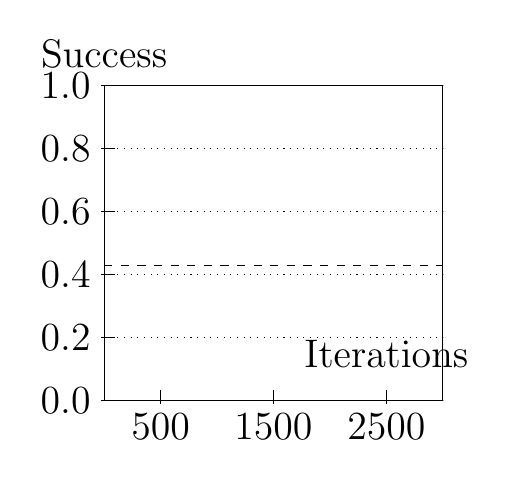
\begin{tikzpicture}[x=0.00143cm,y=4cm]
    % Draw the axes and grid lines
    \draw[-] (0,0) -- (0,1) -- (3000,1) -- (3000,0) -- cycle; 
    \draw[-,thin, dotted, ystep=0.2, xstep=3000] (0,0) grid (3000,1);
    \foreach \x in {500, 1500, 2500}  \draw [-,xshift=0](\x,4pt) -- (\x,-1pt);
    \foreach \y in {0.0,0.2,0.4,0.6,0.8,1.0}  \draw [-,yshift=0](4pt,\y) -- (-1pt,\y);
    \foreach \x/\xtext in {500/500, 1500/1500, 2500/2500} \node at (\x,0) [below] {$\xtext$};
    \foreach \y/\ytext in {0.0,0.2,0.4,0.6,0.8,1.0}  \node at (0,\y) [left] {$\ytext$};
    \node at (0,1.1) {Success};
    \node at (2500,0.15) {Iterations};
    \draw[-] plot[mark=triangle,gray,mark size=3,mark options={color=gray}] 
			file {data/test05v3gm.CP.tikzdata};
    \draw[-] plot[mark=o,gray,mark size=2,mark options={color=gray}] 
			file {data/test05v3gm.SP.tikzdata};
    % Also draw the expected convergence: 0.9^8 actions=0.43046
    \draw[dashed,-,yshift=0](0,0.43046) -- (3000,0.43046);

\end{tikzpicture}

%!TEX root = ../dsingh-aamas10-poster.tex
\begin{tikzpicture}[x=0.0032cm,y=9cm]
    % Draw the axes and grid lines
    \draw[-] (0,0) -- (0,1) -- (5000,1) -- (5000,0) -- cycle; 
    \draw[-,thin, dotted, ystep=0.2, xstep=5000] (0,0) grid (5000,1);
    \foreach \x in {1000, 2500, 4000}  \draw [-,xshift=0](\x,4pt) -- (\x,-1pt);
    \foreach \y in {0.0,0.2,0.4,0.6,0.8,1.0}  \draw [-,yshift=0](4pt,\y) -- (-1pt,\y);
    \foreach \x/\xtext in {1000/1000, 2500/2500, 4000/4000} \node at (\x,0) [below] {\xtext};
    \foreach \y/\ytext in {0.0,0.2,0.4,0.6,0.8,1.0}  \node at (0,\y) [left] {\ytext};
    \node at (0,1.15) {Success};
    \node at (4150,0.1) {Iterations};
    \draw[-,red] plot[mark=x,mark size=10,mark options={color=red}] 
			file {figs/data/testImpactvars2.CP.tikzdata};
    \draw[-,blue] plot[mark=o,mark size=6,mark options={color=blue}] 
			file {figs/data/testImpactvars2.SP.tikzdata};
    % Also draw the expected convergence: 0.9^4 actions=0.6561
    \draw[dashed,-,yshift=0](0,0.6561) -- (5000,0.6561);
	\node at (5700,0.5) {$\mathcal{T}3$};

\end{tikzpicture}

%!TEX root = ../dsingh-aamas10-poster.tex
\begin{tikzpicture}[x=0.00533cm,y=6cm]
    % Draw the axes and grid lines
    \draw[-] (0,-0.25) -- (0,1.25) -- (3000,1.25) -- (3000,-0.25) -- cycle; 
    \draw[-,thin, dotted, ystep=0.25, xstep=3000] (0,-0.25) grid (3000,1.25);
    \foreach \x in {500, 1500, 2500}  \draw [-,xshift=0,yshift=-0.25](\x,-0.20) -- (\x,-0.25);
    \foreach \y in {-0.25,0.00,0.25,0.50,0.75,1.00,1.25}  \draw [-,yshift=0](4pt,\y) -- (-1pt,\y);
    \foreach \x/\xtext in {500/500, 1500/1500, 2500/2500} \node at (\x,-0.25) [below] {\xtext};
    \foreach \y/\ytext in {0.00,0.25,0.50,0.75,1.00}  \node at (0,\y) [left] {\ytext};
    \node at (-70,1.45) {Success};
    \node at (2500,-0.1) {Iterations};
    \draw[-,red] plot[mark=x,mark size=4,mark options={color=red}] 
			file {figs/data/test05v3gmt.CC.tikzdata};
    \draw[-,thin,densely dashed,black] plot[mark=x,mark size=4,mark options={color=black}] 
			file {figs/data/test05v3gmt.CP.tikzdata};
    \draw[-,thin,densely dashed,black] plot[mark=o,mark size=2,mark options={color=black}] 
			file {figs/data/test05v3gmt.SP.tikzdata};
    % Also draw the expected convergence: 0.9^8 actions=0.43046
    \draw[dashed,-,yshift=0](0,1.0) -- (3000,1.0);
	\node at (3500,0.5) {$\mathcal{T}2,20\%$};

\end{tikzpicture}

\end{center}
\vskip -0.5em

The above results compare performance of\\ {\color{darkred}ACL+coverage (crosses)} and {\color{darkblue}BUL (circles)}\\ for various goal-plan hierarchies.

\end{textblock}


%%%%% Footer
\begin{textblock}{15}(0,24)
\begin{center}
\color{darkred}{\LARGE
D.~Singh, S.~Sardina, L.~Padgham, S.~Airiau, Learning context conditions for
  {BDI} plan selection. In {\it Proceedings of Autonomous Agents and Multi-Agent
  Systems (AAMAS)}, Toronto, Canada, 2010.
}
\end{center}
\end{textblock}

\end{document}